\documentclass[11pt,a4paper]{article}
\usepackage[margin=1in]{geometry}
\usepackage[T1]{fontenc}
\usepackage[utf8]{inputenc}
\usepackage{lmodern}
\usepackage{microtype}
\usepackage{amsthm,amsmath,amssymb,amsfonts}
\usepackage{mathtools}
\usepackage{tikz}
\usetikzlibrary{decorations.pathreplacing}

% Long jobs are red, short jobs blue, separators amber, and grid lines gray.
\definecolor{myred}{rgb}{0.75,0,0}
\definecolor{myblue}{rgb}{0,0,0.72}
\definecolor{mygreen}{rgb}{0,0.5,0}
\definecolor{mysolutioncolor}{rgb}{0.72,0.52,0}
\definecolor{mygray}{rgb}{0.55,0.55,0.55}
\usepackage[colorlinks,urlcolor=blue!50!black,linkcolor=blue!50!black,citecolor=green!40!black]{hyperref}

\newtheorem{theorem}{Theorem}
\newtheorem{lemma}{Lemma}
\newtheorem{proposition}{Proposition}
\newtheorem{observation}{Observation}
\theoremstyle{definition}
\newtheorem{definition}{Definition}
\newtheorem{construction}{Construction}

\newcommand{\AUX}{\textsc{Aux}}
\newcommand{\pmax}{p_{\max}}
\newcommand{\phash}{\#P}
\newcommand{\LMAX}{L_{\max}}
\newcommand{\NP}{\textnormal{\textsf{NP}}}
\newcommand{\SAT}{\textsc{Sat}}

\title{Scheduling with Two Non-Unit Job Lengths Is NP-Complete}
\author{Yuval Itzhaki \and Claude}
\date{}

\begin{document}
\maketitle

\begin{abstract}
This work formalizes a theorem of Elffers and de Weerdt~\cite{EdW17}:
non-preemptive scheduling of jobs with release times and deadlines on a single
machine, $1\mid r_j\mid\LMAX$, is polynomial-time solvable when all jobs have the
same length, and when the jobs have two lengths of which the shorter is
$1$~\cite{Sgall12}. Elffers and de Weerdt settle the remaining case: for every fixed pair of integer
job lengths $p>q>1$, the problem restricted to the job lengths $\{p,q\}$ is
NP-complete. The reduction produces only numbers polynomial in the size of the
input, which is why they call the problem strongly NP-complete.
\end{abstract}

\section{The Problem}

A single machine processes $n$ jobs, one at a time and without preemption.
Job $j$ carries a release time $r_j$, a deadline $d_j$, and a processing time
$p_j$, all non-negative integers.

\begin{definition}[Scheduling with Release Times and Deadlines]
\label{def:scheduling}
% lax begin Lax391470.Scheduling
An \emph{instance} is a finite set of jobs~$\big([r_j,d_j],p_j\big)$. A
\emph{schedule} is a start-time assignment $t$; it is \emph{feasible} if
every job runs inside its availability window,
\[
  r_j \;\le\; t(j) \;\le\; d_j - p_j \qquad\text{for every job } j,
\]
and the jobs' execution intervals $[t(j),\,t(j)+p_j)$ are pairwise disjoint.
An instance is \emph{schedulable} if it admits a feasible schedule.
% lax end
\end{definition}

Figure~\ref{fig:instance} shows a feasible schedule of a two-job instance.

\begin{figure}[h]
\centering
% A small scheduling instance: four jobs, their availability windows, and
% one feasible placement. Redrawn, with the talk's own colors, from the
% slide "Single Machine Scheduling Release Times" of
% OneRjLmax/talk/rjlmax-talk.tex.
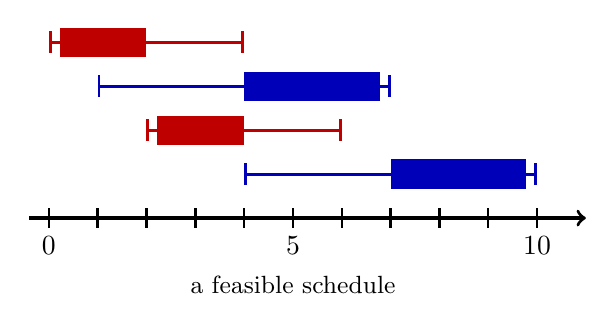
\begin{tikzpicture}[x=0.62cm,y=0.62cm]
  \draw[myred,line width=1.pt,|-|]  (0,3.6) -- (4,3.6);
    \fill[myred] (0.22,3.3) rectangle (2,3.9);
  \draw[myblue,line width=1.pt,|-|] (1,2.7) -- (7,2.7);
    \fill[myblue] (4,2.4) rectangle (6.78,3.0);
  \draw[myred,line width=1.pt,|-|]  (2,1.8) -- (6,1.8);
    \fill[myred] (2.22,1.5) rectangle (4,2.1);
  \draw[myblue,line width=1.pt,|-|] (4,0.9) -- (10,0.9);
    \fill[myblue] (7,0.6) rectangle (9.78,1.2);
  \draw[line width=1.2pt,->] (-0.4,0) -- (11,0);
  \foreach \x in {0,...,10} \draw[line width=.9pt] (\x,-0.2) -- (\x,0.2);
  \foreach \x in {0,5,10} \node[font=\normalsize,anchor=north] at (\x,-0.18) {\x};
  \node[font=\small,anchor=north] at (5,-1.0) {a feasible schedule};
\end{tikzpicture}

\caption{Two jobs, their availability windows, and one feasible placement.}
\label{fig:instance}
\end{figure}

A feasible schedule exists exactly when $\LMAX\le 0$ for the usual
maximum-lateness objective, which in turn holds exactly when every job can be
made on time, $\sum_j U_j = 0$; this is the sense in which the decision
problem above is $1\mid r_j\mid\LMAX$.

Elffers and de Weerdt organize the complexity landscape of this problem
around the \emph{set of lengths that occur}, $P(S)=\{p_j : j\in S\}$: the
number of distinct lengths, $\phash:=|P(S)|$, and the longest length,
$\pmax:=\max P(S)$. The general problem is strongly NP-hard by a reduction
from \textsc{3-Partition}, so the interesting question is how small $P(S)$
can be made before the problem turns easy. A single length ($\phash=1$) is
trivially polynomial; two lengths of which the shorter is $1$ is also
polynomial, by an LP-rounding algorithm of Sgall~\cite{Sgall12}. Elffers and
de Weerdt's remaining case, two lengths neither of them $1$, is the subject
of this formalization.

Sgall's survey of open problems in throughput scheduling poses exactly this
question: is there a polynomial-time algorithm for $1\mid r_j,\,p_j\le
c\mid\sum U_j$ for constant $c$, i.e.\ does $P(S)$ staying small enough keep
the problem easy~\cite{Sgall12}? Mnich and van Bevern's survey of
parameterized machine scheduling restates it as Open Problem 3: are
$1\mid r_j\mid\sum U_j$ and $1\mid r_j\mid\sum w_jU_j$
\textnormal{\textsf{W[1]}}-hard parameterized by $\pmax$, membership in even
\textnormal{\textsf{XP}} being open~\cite{Mnich18}. Taking $p=2q$ in
Theorem~\ref{thm:main}, for every $q\ge 2$, contradicts Vakhania's claimed
pseudo-polynomial algorithm for $p_j\in\{q,2q\}$~\cite{Vakhania04}.

\section{The Main Theorem}

Instances are read as finite binary words: a natural number is its digits
preceded by their count in unary, and a scheduling instance is the
concatenation of its jobs' numbers, each number's sign bit first.

\begin{definition}[Instances as Words]
\label{def:encoding}
% lax begin Lax391470.BinaryEncoding
\emph{Scheduling on the lengths $\{p,q\}$}, for fixed $p,q$, is the language
of binary words encoding an instance all of whose processing times lie in
$\{p,q\}$ and which is schedulable.
% lax end
\end{definition}

\begin{theorem}[Elffers--de Weerdt]
\label{thm:main}
% lax begin Lax391470.Theorem1
Let $p>q>1$ be two integer job lengths. Scheduling on the lengths $\{p,q\}$
is \NP-complete.
% lax end
\end{theorem}

The membership half of Theorem~\ref{thm:main} holds unconditionally, for every pair
of lengths:

\begin{theorem}
% lax begin Lax391470Proofs.V1Final.twoLengths_mem_NP
Scheduling on the lengths $\{p,q\}$ belongs to \NP, for every $p,q$.
% lax end
\end{theorem}

A certificate is a schedule with integer start times; feasibility confines
every start time between a release time and a deadline of the instance, so
the certificate has size polynomial in the instance encoding, and checking it is
immediate. Hardness is the substance of the theorem, and the rest of this
paper is its proof.

\begin{observation}
\label{obs:paranphard}
Since a feasible schedule exists exactly when $\sum_j U_j=0$
(Definition~\ref{def:scheduling}), Theorem~\ref{thm:main} says that $1\mid r_j,\,p_j\le
p\mid\sum U_j$ is \NP-hard already for a \emph{constant} $p$, i.e.\
\textnormal{\textsf{para-NP}}-hard parameterized by $\pmax$. In particular
there is no polynomial-time algorithm for any fixed bound on $\pmax$ unless
$\textsf{P}=\NP$, which settles Sgall's question and Mnich and van Bevern's
Open Problem 3~\cite{Sgall12,Mnich18}.
\end{observation}

\section{The Shape of the Proof}

The reduction from satisfiability does not go directly to scheduling.
Deciding a clause needs a disjunction between two jobs whose deadlines can be
far apart, and plain release times and deadlines cannot say that. Elffers and
de Weerdt introduce an intermediate problem that can.

\begin{figure}[h]
\centering
% The shape of the proof: two reductions composed.
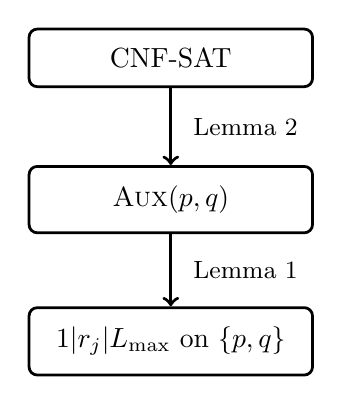
\begin{tikzpicture}[x=1cm,y=1cm,
  box/.style={draw,line width=1pt,rounded corners=3pt,inner sep=7pt,
              minimum width=3.6cm,align=center}]
  \node[box] (sat) at (0,3)   {CNF-SAT};
  \node[box] (aux) at (0,1.2) {$\AUX(p,q)$};
  \node[box] (sch) at (0,-0.6) {$1|r_j|\LMAX$ on $\{p,q\}$};
  \draw[->,line width=1.2pt] (sat) -- (aux)
    node[midway,right=.15cm,font=\small] {Lemma 2};
  \draw[->,line width=1.2pt] (aux) -- (sch)
    node[midway,right=.15cm,font=\small] {Lemma 1};
\end{tikzpicture}

\caption{\SAT{} reduces to the auxiliary problem $\AUX(p,q)$ (Lemma~\ref{lem:lemma2}),
which reduces to scheduling on $\{p,q\}$ (Lemma~\ref{lem:lemma1}).}
\label{fig:shape}
\end{figure}

\begin{definition}[The Auxiliary Problem $\AUX(p,q)$]
\label{def:aux}
% lax begin Lax391470.AuxiliaryProblem
An instance of $\AUX(p,q)$ consists of ordinary jobs as in
Definition~\ref{def:scheduling}, together with $N$ \emph{pending pairs}~$(J_{p,i},J_{q,i})_{i=1}^N$. Both jobs of a pair are released at $0$; $J_{p,i}$
has length $p$ and $J_{q,i}$ has length $q$. Each pending job carries two
deadlines, an \emph{early} one $d'$ and a \emph{late} one $d$, with
$d'\le d$. The instance is \emph{ordered} when, for every $i$,
\[
  d'_{p,i}\le d_{p,i}\le d'_{p,i+1}, \qquad
  d'_{q,i}\le d_{q,i}\le d'_{q,i+1}, \qquad
  d_{p,i}\le d'_{q,i},
\]
and it has a \emph{solution} if there is a feasible schedule with respect to
the late deadlines in which, for every $i$, at least one of $J_{p,i}$,
$J_{q,i}$ meets its early deadline.
% lax end
\end{definition}

Figure~\ref{fig:pair} shows one connected pending pair.

\begin{figure}[h]
\centering
% Two connected pending pairs of AUX(p,q): the long job (red) and the short
% job (blue) of each pair, both released at 0, with the early deadline
% marked by a thick tick. Redrawn, with the talk's own colors, from the
% slide "The Auxiliary Problem AUX(p,q)" of OneRjLmax/talk/rjlmax-talk.tex;
% the deadline labels on pair 1, omitted on the slide itself (left to the
% speaker), are added here.
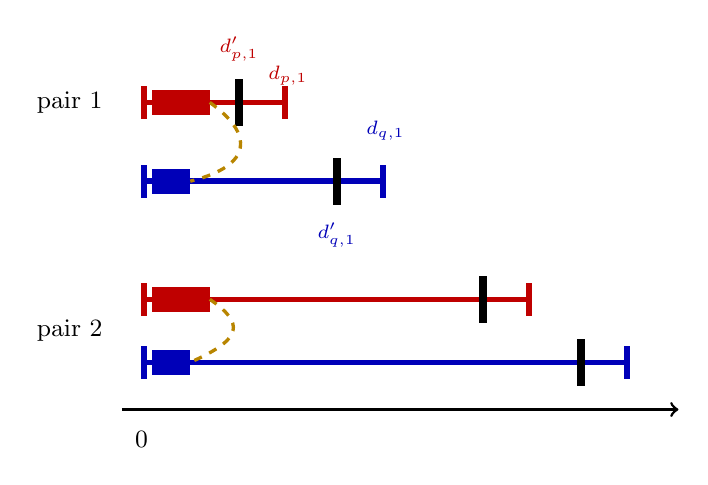
\begin{tikzpicture}[x=0.62cm,y=1.0cm]
  \draw[line width=1pt,->] (-0.4,0) -- (11,0);
  \node[font=\small,anchor=north] at (0,-0.15) {$0$};
  \node[font=\small,anchor=east] at (-0.6,3.9) {pair $1$};
  \draw[myred,line width=2pt,|-|]  (0,3.9) -- (3,3.9);
    \fill[myred] (0.22,3.74) rectangle (1.4,4.06);
    \draw[line width=3pt] (2,3.6) -- (2,4.2);
    \node[font=\scriptsize,text=myred,anchor=south] at (2,4.3) {$d'_{p,1}$};
    \node[font=\scriptsize,text=myred,anchor=south] at (3,4.0) {$d_{p,1}$};
  \draw[myblue,line width=2pt,|-|] (0,2.9) -- (5,2.9);
    \fill[myblue] (0.22,2.74) rectangle (1,3.06);
    \draw[line width=3pt] (4,2.6) -- (4,3.2);
    \node[font=\scriptsize,text=myblue,anchor=north] at (4,2.5) {$d'_{q,1}$};
    \node[font=\scriptsize,text=myblue,anchor=south] at (5,3.3) {$d_{q,1}$};
  \draw[mysolutioncolor,line width=1.2pt,dashed] (1.4,3.9) .. controls (2.3,3.5) and (2.3,3.1) .. (1,2.9);
  \node[font=\small,anchor=east] at (-0.6,1.0) {pair $2$};
  \draw[myred,line width=2pt,|-|]  (0,1.4) -- (8,1.4);
    \fill[myred] (0.22,1.24) rectangle (1.4,1.56);
    \draw[line width=3pt] (7,1.1) -- (7,1.7);
  \draw[myblue,line width=2pt,|-|] (0,0.6) -- (10,0.6);
    \fill[myblue] (0.22,0.44) rectangle (1,0.76);
    \draw[line width=3pt] (9,0.3) -- (9,0.9);
  \draw[mysolutioncolor,line width=1.2pt,dashed] (1.4,1.4) .. controls (2.1,1.1) and (2.1,0.9) .. (1,0.6);
\end{tikzpicture}

\caption{A connected pending pair: at least one of the two jobs must meet
its early deadline.}
\label{fig:pair}
\end{figure}

\section{From Satisfiability to $\AUX(p,q)$}

\setcounter{lemma}{1}
\begin{lemma}
\label{lem:lemma2}
% lax begin Lax391470.Lemma2
For job lengths $p>q>1$, $\AUX(p,q)$ is \NP-complete; the reduction from
every language in \NP{} factors through a polynomial-time many-one reduction
from satisfiability.
% lax end
\end{lemma}

\begin{proof}[Construction]
% lax begin Lax391470.SatConstruction
Fix a CNF formula $F$ with $n$ variables and $m$ clauses
$C_0,\dots,C_{m-1}$. The time line is cut into $2n$ \emph{sections} of equal
length $S=(p+2q)+m(p+q)+1+q$, one for every literal, in the order
$x_0,\neg x_0,x_1,\neg x_1,\dots$ A section consists of a \emph{literal
block} of total job length $p+2q$, then one \emph{clause block} of total job
length $p+q$ for every clause, then one unit of idle time, then a
\emph{separator}: an ordinary short job pinned to the last $q$ time units of
the section.
% lax end
Within a literal block, the jobs are arranged so that a feasible schedule has
exactly two shapes, differing by one unit of idle time: one shape leaves no
idle time in the block and corresponds to the literal being \textsc{true}, the
other leaves exactly one unit of idle time and corresponds to \textsc{false}.
A short ordinary job of length $q\ge 2$ cannot absorb that one unit of slack
on its own, so the idle time, once created, propagates rightwards through
every clause block that follows in the section: a clause block lets the slack
through unless one of its literals is set to make the clause true, in which
case the block's pending pair is tethered so as to absorb it. A clause is
satisfied exactly when some literal's block feeds its clause block enough
slack to stop the propagation before it reaches the separator, which is why
the separator's own feasibility encodes satisfiability of the whole formula.

Figure~\ref{fig:blocks} shows all four block shapes: the selection gadgets $V^+$,
$V^-$ for a positive and a negative literal, and the clause gadgets
$C_{\text{act}}$, $C_{\text{inact}}$ for a clause that does, respectively
does not, contain that literal.

\begin{figure}[ht]
\centering
% The four block shapes a section is built from: the selection gadgets for
% a positive and a negative literal, and the clause gadgets for a clause
% that does, respectively does not, contain that literal. Each gadget is
% shown in the state where its slack is absorbed (no idle time reaches the
% separator) except $V^-$ and $C_{\text{inact}}$, shown with their one unit
% of idle time, together illustrating one full literal assignment and one
% satisfied, one unsatisfied clause slot. Redrawn, with the talk's own
% colors, from the slide "The Four Blocks" of
% OneRjLmax/talk/rjlmax-talk.tex.
\begin{minipage}[t]{0.5\textwidth}
\centering
\textbf{$V^{+}$}: literal $x_i$, no idle time

\vspace{.08cm}
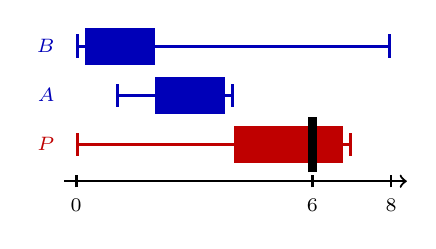
\begin{tikzpicture}[x=0.5cm,y=0.78cm]
  \draw[myblue,line width=1.1pt,|-|] (0,2.2) -- (8,2.2);
    \node[font=\scriptsize,anchor=east,text=myblue] at (-0.3,2.2) {$B$};
  \draw[myblue,line width=1.1pt,|-|] (1,1.4) -- (4,1.4);
    \node[font=\scriptsize,anchor=east,text=myblue] at (-0.3,1.4) {$A$};
  \draw[myred,line width=1.1pt,|-|] (0,0.6) -- (7,0.6);
    \node[font=\scriptsize,anchor=east,text=myred] at (-0.3,0.6) {$P$};
  \draw[line width=.8pt,->] (-0.3,0) -- (8.4,0);
    \foreach \tx/\tl in {0/0,6/6,8/8} {
      \draw[line width=1pt] (\tx,-0.1) -- (\tx,0.1);
      \node[font=\scriptsize,anchor=north] at (\tx,-0.13) {$\tl$};}
  \fill[myblue] (0.22,1.9) rectangle (2,2.5);
  \fill[myblue] (2,1.1)    rectangle (3.78,1.7);
  \fill[myred]  (4,0.3)    rectangle (6.78,0.9);
  \draw[line width=3pt] (6,0.15) -- (6,1.05);
\end{tikzpicture}
\end{minipage}%
\begin{minipage}[t]{0.5\textwidth}
\centering
\textbf{$V^{-}$}: literal $\neg x_i$, one unit idle

\vspace{.08cm}
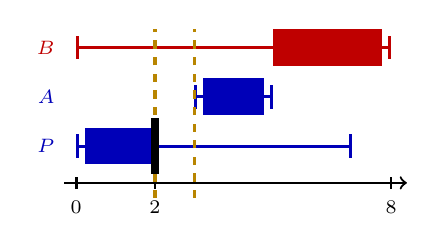
\begin{tikzpicture}[x=0.5cm,y=0.78cm]
  \draw[myred,line width=1.1pt,|-|]  (0,2.2) -- (8,2.2);
    \node[font=\scriptsize,anchor=east,text=myred] at (-0.3,2.2) {$B$};
  \draw[myblue,line width=1.1pt,|-|] (3,1.4) -- (5,1.4);
    \node[font=\scriptsize,anchor=east,text=myblue] at (-0.3,1.4) {$A$};
  \draw[myblue,line width=1.1pt,|-|] (0,0.6) -- (7,0.6);
    \node[font=\scriptsize,anchor=east,text=myblue] at (-0.3,0.6) {$P$};
  \draw[line width=.8pt,->] (-0.3,0) -- (8.4,0);
    \foreach \tx/\tl in {0/0,2/2,8/8} {
      \draw[line width=1pt] (\tx,-0.1) -- (\tx,0.1);
      \node[font=\scriptsize,anchor=north] at (\tx,-0.13) {$\tl$};}
  \draw[mysolutioncolor,line width=1.2pt,dashed] (2,-0.25) -- (2,2.5);
  \draw[mysolutioncolor,line width=1.2pt,dashed] (3,-0.25) -- (3,2.5);
  \fill[myblue] (0.22,0.3) rectangle (2,0.9);
  \fill[myblue] (3.22,1.1) rectangle (4.78,1.7);
  \fill[myred]  (5,1.9)    rectangle (7.78,2.5);
  \draw[line width=3pt] (2,0.15) -- (2,1.05);
\end{tikzpicture}
\end{minipage}

\vspace{.2cm}

\begin{minipage}[t]{0.5\textwidth}
\centering
\textbf{$C_{\text{act}}$}: clause \emph{has} the literal

\vspace{.08cm}
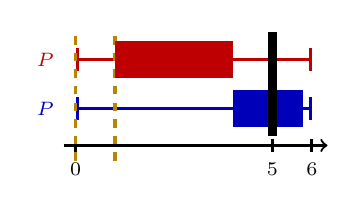
\begin{tikzpicture}[x=0.5cm,y=0.78cm]
  \draw[myred,line width=1.1pt,|-|]  (0,1.4) -- (6,1.4);
    \node[font=\scriptsize,anchor=east,text=myred] at (-0.3,1.4) {$P$};
  \draw[myblue,line width=1.1pt,|-|] (0,0.6) -- (6,0.6);
    \node[font=\scriptsize,anchor=east,text=myblue] at (-0.3,0.6) {$P$};
  \draw[line width=.8pt,->] (-0.3,0) -- (6.4,0);
    \foreach \tx/\tl in {0/0,5/5,6/6} {
      \draw[line width=1pt] (\tx,-0.1) -- (\tx,0.1);
      \node[font=\scriptsize,anchor=north] at (\tx,-0.13) {$\tl$};}
  \draw[mysolutioncolor,line width=1.2pt,dashed] (0,-0.25) -- (0,1.85);
  \draw[mysolutioncolor,line width=1.2pt,dashed] (1,-0.25) -- (1,1.85);
  \fill[myred]  (1,1.1) rectangle (4,1.7);
  \fill[myblue] (4,0.3) rectangle (5.78,0.9);
  \draw[line width=3pt] (5,0.95) -- (5,1.85);
  \draw[line width=3pt] (5,0.15) -- (5,1.05);
\end{tikzpicture}
\end{minipage}%
\begin{minipage}[t]{0.5\textwidth}
\centering
\textbf{$C_{\text{inact}}$}: clause \emph{misses} it

\vspace{.08cm}
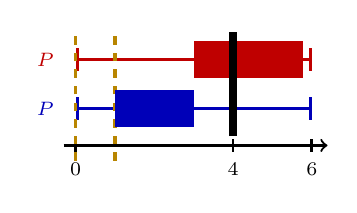
\begin{tikzpicture}[x=0.5cm,y=0.78cm]
  \draw[myred,line width=1.1pt,|-|]  (0,1.4) -- (6,1.4);
    \node[font=\scriptsize,anchor=east,text=myred] at (-0.3,1.4) {$P$};
  \draw[myblue,line width=1.1pt,|-|] (0,0.6) -- (6,0.6);
    \node[font=\scriptsize,anchor=east,text=myblue] at (-0.3,0.6) {$P$};
  \draw[line width=.8pt,->] (-0.3,0) -- (6.4,0);
    \foreach \tx/\tl in {0/0,4/4,6/6} {
      \draw[line width=1pt] (\tx,-0.1) -- (\tx,0.1);
      \node[font=\scriptsize,anchor=north] at (\tx,-0.13) {$\tl$};}
  \draw[mysolutioncolor,line width=1.2pt,dashed] (0,-0.25) -- (0,1.85);
  \draw[mysolutioncolor,line width=1.2pt,dashed] (1,-0.25) -- (1,1.85);
  \fill[myblue] (1,0.3) rectangle (3,0.9);
  \fill[myred]  (3,1.1) rectangle (5.78,1.7);
  \draw[line width=3pt] (4,0.95) -- (4,1.85);
  \draw[line width=3pt] (4,0.15) -- (4,1.05);
\end{tikzpicture}
\end{minipage}

\caption{The four block shapes. $B$, $A$, $P$ are ordinary jobs; the two
rows marked $P$ in a clause gadget are the pending jobs of its connected
pair, as in Figure~\ref{fig:pair}.}
\label{fig:blocks}
\end{figure}

Complementary literals $x_i,\neg x_i$ are kept consistent by a connected
pending pair tethering their two literal blocks, so that one is forced
\textsc{true} exactly when the other is forced \textsc{false}.
Figure~\ref{fig:gadgets} assembles four full sections, $x_1,\neg x_1,x_2,\neg
x_2$, for the formula $(x_1\lor x_2)\land(\neg x_1\lor x_2)$, every
tethered pair shown.

\begin{figure}[ht]
\centering
\resizebox{\textwidth}{!}{% Four full sections of the construction: x_1, neg x_1, x_2, neg x_2, for
% the formula (x_1 or x_2) and (neg x_1 or x_2). Every job is drawn, none
% collapsed into a single representative bar. Dashed lines mark connected
% pairs: between a variable's two literal blocks, and along each clause's
% chain of clause blocks. Redrawn, with the talk's own colors, from the
% slide "The Gadget Layout" of OneRjLmax/talk/rjlmax-talk.tex.
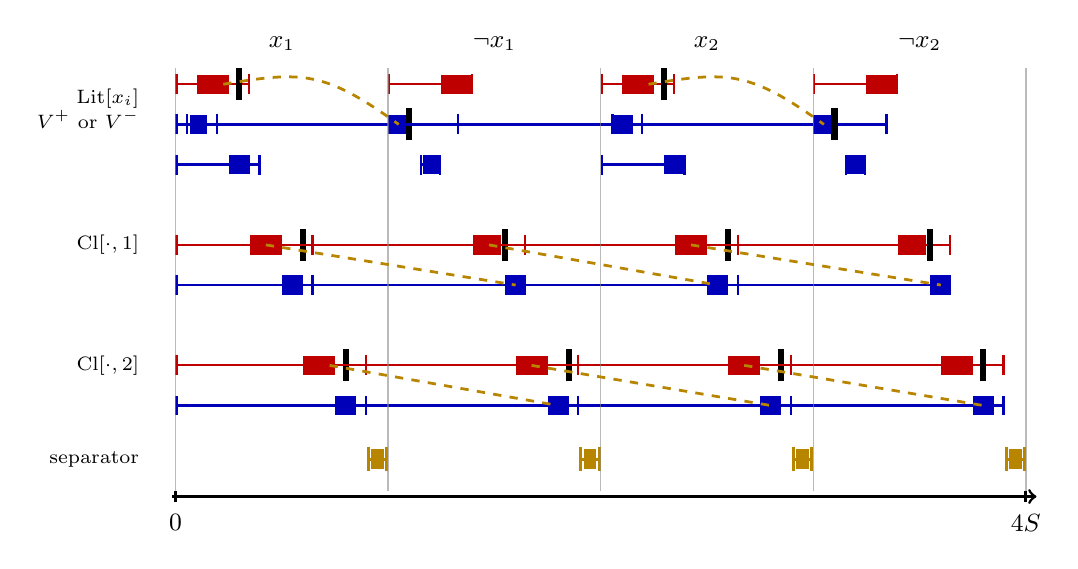
\begin{tikzpicture}[x=0.135cm,y=0.68cm]
  \node[font=\scriptsize,anchor=east,align=right] at (-2.5,6.25) {$\mathrm{Lit}[x_i]$\\$V^+$ or $V^-$};
  \node[font=\scriptsize,anchor=east] at (-2.5,3.7) {$\mathrm{Cl}[\cdot,1]$};
  \node[font=\scriptsize,anchor=east] at (-2.5,1.45) {$\mathrm{Cl}[\cdot,2]$};
  \node[font=\scriptsize,anchor=east] at (-2.5,-0.3) {separator};
  %% ---- x_1 (o=0): V+, Cl1=act, Cl2=inact ----
  \draw[myred,line width=.8pt,|-|]  (0,6.7) -- (7,6.7);
    \draw[line width=2.2pt] (6,6.4) -- (6,7);
    \fill[myred] (2,6.52) rectangle (5,6.88);
  \draw[myblue,line width=.8pt,|-|] (1,5.95) -- (4,5.95);
    \fill[myblue] (1.35,5.77) rectangle (3,6.13);
  \draw[myblue,line width=.8pt,|-|] (0,5.2) -- (8,5.2);
    \fill[myblue] (5,5.02) rectangle (7,5.38);
  \draw[myred,line width=.8pt,|-|]  (0,3.7) -- (13,3.7);
    \draw[line width=2.2pt] (12,3.4) -- (12,4);
    \fill[myred] (7,3.52) rectangle (10,3.88);
  \draw[myblue,line width=.8pt,|-|] (0,2.95) -- (13,2.95);
    \fill[myblue] (10,2.77) rectangle (12,3.13);
  \draw[myred,line width=.8pt,|-|]  (0,1.45) -- (18,1.45);
    \draw[line width=2.2pt] (16,1.15) -- (16,1.75);
    \fill[myred] (12,1.27) rectangle (15,1.63);
  \draw[myblue,line width=.8pt,|-|] (0,0.7) -- (18,0.7);
    \fill[myblue] (15,0.52) rectangle (17,0.88);
  \draw[mysolutioncolor,line width=1.1pt,|-|] (18,-0.3) -- (20,-0.3);
    \fill[mysolutioncolor] (18.4,-0.48) rectangle (19.6,-0.12);
  \node[font=\small,anchor=south] at (10,7.15) {$x_1$};
  %% ---- neg x_1 (o=20): V-, Cl1=inact, Cl2=act ----
  \draw[myred,line width=.8pt,|-|]  (20,6.7) -- (28,6.7);
    \fill[myred] (25,6.52) rectangle (27.85,6.88);
  \draw[myblue,line width=.8pt,|-|] (0,5.95) -- (26.65,5.95);
    \draw[line width=2.2pt] (22,5.65) -- (22,6.25);
    \fill[myblue] (20,5.77) rectangle (21.65,6.13);
  \draw[myblue,line width=.8pt,|-|] (23,5.2) -- (25,5.2);
    \fill[myblue] (23.25,5.02) rectangle (24.75,5.38);
  \draw[myred,line width=.8pt,|-|]  (0,3.7) -- (33,3.7);
    \draw[line width=2.2pt] (31,3.4) -- (31,4);
    \fill[myred] (28,3.52) rectangle (30.65,3.88);
  \draw[myblue,line width=.8pt,|-|] (0,2.95) -- (33,2.95);
    \fill[myblue] (31,2.77) rectangle (32.85,3.13);
  \draw[myred,line width=.8pt,|-|]  (0,1.45) -- (38,1.45);
    \draw[line width=2.2pt] (37,1.15) -- (37,1.75);
    \fill[myred] (32,1.27) rectangle (35,1.63);
  \draw[myblue,line width=.8pt,|-|] (0,0.7) -- (38,0.7);
    \fill[myblue] (35,0.52) rectangle (37,0.88);
  \draw[mysolutioncolor,line width=1.1pt,|-|] (38,-0.3) -- (40,-0.3);
    \fill[mysolutioncolor] (38.4,-0.48) rectangle (39.6,-0.12);
  \node[font=\small,anchor=south] at (30,7.15) {$\neg x_1$};
  %% ---- x_2 (o=40): V+, Cl1=act, Cl2=act ----
  \draw[myred,line width=.8pt,|-|]  (40,6.7) -- (47,6.7);
    \draw[line width=2.2pt] (46,6.4) -- (46,7);
    \fill[myred] (42,6.52) rectangle (45,6.88);
  \draw[myblue,line width=.8pt,|-|] (41,5.95) -- (44,5.95);
    \fill[myblue] (41.15,5.77) rectangle (43,6.13);
  \draw[myblue,line width=.8pt,|-|] (40,5.2) -- (48,5.2);
    \fill[myblue] (46,5.02) rectangle (47.85,5.38);
  \draw[myred,line width=.8pt,|-|]  (0,3.7) -- (53,3.7);
    \draw[line width=2.2pt] (52,3.4) -- (52,4);
    \fill[myred] (47,3.52) rectangle (50,3.88);
  \draw[myblue,line width=.8pt,|-|] (0,2.95) -- (53,2.95);
    \fill[myblue] (50,2.77) rectangle (52,3.13);
  \draw[myred,line width=.8pt,|-|]  (0,1.45) -- (58,1.45);
    \draw[line width=2.2pt] (57,1.15) -- (57,1.75);
    \fill[myred] (52,1.27) rectangle (55,1.63);
  \draw[myblue,line width=.8pt,|-|] (0,0.7) -- (58,0.7);
    \fill[myblue] (55,0.52) rectangle (57,0.88);
  \draw[mysolutioncolor,line width=1.1pt,|-|] (58,-0.3) -- (60,-0.3);
    \fill[mysolutioncolor] (58.4,-0.48) rectangle (59.6,-0.12);
  \node[font=\small,anchor=south] at (50,7.15) {$x_2$};
  %% ---- neg x_2 (o=60): V-, Cl1=inact, Cl2=inact ----
  \draw[myred,line width=.8pt,|-|]  (60,6.7) -- (68,6.7);
    \fill[myred] (65,6.52) rectangle (67.85,6.88);
  \draw[myblue,line width=.8pt,|-|] (0,5.95) -- (67,5.95);
    \draw[line width=2.2pt] (62,5.65) -- (62,6.25);
    \fill[myblue] (60,5.77) rectangle (61.65,6.13);
  \draw[myblue,line width=.8pt,|-|] (63,5.2) -- (65,5.2);
    \fill[myblue] (63.15,5.02) rectangle (64.85,5.38);
  \draw[myred,line width=.8pt,|-|]  (0,3.7) -- (73,3.7);
    \draw[line width=2.2pt] (71,3.4) -- (71,4);
    \fill[myred] (68,3.52) rectangle (70.65,3.88);
  \draw[myblue,line width=.8pt,|-|] (0,2.95) -- (73,2.95);
    \fill[myblue] (71,2.77) rectangle (72.85,3.13);
  \draw[myred,line width=.8pt,|-|]  (0,1.45) -- (78,1.45);
    \draw[line width=2.2pt] (76,1.15) -- (76,1.75);
    \fill[myred] (72,1.27) rectangle (75,1.63);
  \draw[myblue,line width=.8pt,|-|] (0,0.7) -- (78,0.7);
    \fill[myblue] (75,0.52) rectangle (77,0.88);
  \draw[mysolutioncolor,line width=1.1pt,|-|] (78,-0.3) -- (80,-0.3);
    \fill[mysolutioncolor] (78.4,-0.48) rectangle (79.6,-0.12);
  \node[font=\small,anchor=south] at (70,7.15) {$\neg x_2$};
  %% ---- axis, with a tick at every section boundary ----
  \draw[mygray,line width=.5pt,opacity=.6] (0,-0.9)  -- (0,7.0);
  \draw[mygray,line width=.5pt,opacity=.6] (20,-0.9) -- (20,7.0);
  \draw[mygray,line width=.5pt,opacity=.6] (40,-0.9) -- (40,7.0);
  \draw[mygray,line width=.5pt,opacity=.6] (60,-0.9) -- (60,7.0);
  \draw[mygray,line width=.5pt,opacity=.6] (80,-0.9) -- (80,7.0);
  \draw[line width=1pt,->] (-0.3,-1.0) -- (81,-1.0);
    \draw[line width=1pt] (0,-1.1)  -- (0,-0.9);
    \draw[line width=1pt] (80,-1.1) -- (80,-0.9);
    \node[font=\small,anchor=north] at (0,-1.15)  {$0$};
    \node[font=\small,anchor=north] at (80,-1.15) {$4S$};
  % literal pairs: a variable's two literal blocks are connected
  \draw[mysolutioncolor,line width=1pt,dashed] (4.5,6.7) .. controls (12,6.95) and (14,6.95) .. (21,5.95);
  \draw[mysolutioncolor,line width=1pt,dashed] (44.5,6.7) .. controls (52,6.95) and (54,6.95) .. (61,5.95);
  % clause 1's chain
  \draw[mysolutioncolor,line width=1pt,dashed] (8.5,3.7) -- (32,2.95);
  \draw[mysolutioncolor,line width=1pt,dashed] (29.5,3.7) -- (51,2.95);
  \draw[mysolutioncolor,line width=1pt,dashed] (48.5,3.7) -- (72,2.95);
  % clause 2's chain
  \draw[mysolutioncolor,line width=1pt,dashed] (14.5,1.45) -- (36,0.7);
  \draw[mysolutioncolor,line width=1pt,dashed] (33.5,1.45) -- (56,0.7);
  \draw[mysolutioncolor,line width=1pt,dashed] (53.5,1.45) -- (76,0.7);
\end{tikzpicture}
}
\caption{Four sections of the construction for $p=3$, $q=2$: two
variables, each contributing a satisfied and an unsatisfied clause slot to
the two clauses of $(x_1\lor x_2)\land(\neg x_1\lor x_2)$.}
\label{fig:gadgets}
\end{figure}

Correctness is proved as two separate statements:
\begin{itemize}
\item % lax begin Lax391470Proofs.Reduce.lemma2_reduce_correct
    a word belongs to \SAT{} if and only if its image under the reduction
    belongs to $\AUX(p,q)$;
  % lax end
\item % lax begin Lax391470Proofs.SatNumbering.ordered
    the constructed instance is ordered, so that Definition~\ref{def:aux}'s hypothesis
    is met;
  % lax end
\end{itemize}
the forward and converse directions of the first statement are themselves
separate proofs,
% lax begin Lax391470Proofs.SatNumbering.solvable_of_satisfiable
satisfiable $\Rightarrow$ solvable
% lax end
and
% lax begin Lax391470Proofs.SatNumbering.satisfiable_of_solvable
solvable $\Rightarrow$ satisfiable.
% lax end
\end{proof}

\begin{proposition}[The Numbers Stay Small]
\label{prop:sattimes}
% lax begin Lax391470Proofs.SatTimes.times_le
Every release time, deadline, and early or late deadline of the constructed
instance is at most $2nS$, the length of the time line, a polynomial in
the size of the formula.
% lax end
\end{proposition}

Membership of $\AUX(p,q)$ in \NP, and the polynomial running time of the
reduction, are proved by exhibiting word-RAM programs:
% lax begin Lax391470Proofs.V2Final.aux_mem_NP
a verifier for $\AUX(p,q)$ running in polynomial time,
% lax end
and
% lax begin Lax391470Proofs.L2Final.reduce_polyTime
the reduction itself running in polynomial time.
% lax end
Composing these with Cook--Levin gives
% lax begin Lax391470Proofs.Hardness.aux_npHard
NP-hardness of $\AUX(p,q)$,
% lax end
and, with membership,
% lax begin Lax391470Proofs.Hardness.aux_npComplete
its NP-completeness.
% lax end

\section{From $\AUX(p,q)$ to Scheduling}

\setcounter{lemma}{0}
\begin{lemma}
\label{lem:lemma1}
% lax begin Lax391470.Lemma1
For job lengths $p>q\ge 1$, $\AUX(p,q)$ is polynomial-time reducible to
scheduling on the lengths $\{p,q\}$.
% lax end
\end{lemma}

\begin{proof}[Construction]
% lax begin Lax391470.StackedConstruction
Fix $w=q$ and let $t_i=-(p+q+w)\,i$ for $i=1,\dots,N$. For every pending
pair $i$ the constructed instance contains five jobs: a \emph{separator}
with availability interval $[t_i+p+q,\,t_i+p+q+w]$ and length $w$, which is
thereby pinned in place; an \emph{inner} long job~$\big([t_i+q,\,d'_{p,i}],\,p\big)$
and an \emph{outer} long job~$\big([t_i,\,d_{p,i}],\,p\big)$; an \emph{inner}
short job~$\big([t_i+p,\,d'_{q,i}],\,q\big)$ and an \emph{outer} short
job~$\big([t_i,\,d_{q,i}],\,q\big)$. The ordinary jobs are kept unchanged.
% lax end
The separators cut the time before $0$ into $N$ \emph{bins}, each with room
for exactly one long and one short job; the four jobs of a pair are nested,
with the inner ones carrying the early deadlines. A feasible schedule parks
two jobs of each pair in its bin and runs the other two, one long and one
short, after time $0$. The inner long job and the inner short job of a pair
do not both fit into the bin together, so one of the two jobs running after
$0$ is an inner job and meets an early deadline: exactly
Definition~\ref{def:aux}'s condition on connected pairs.

Figure~\ref{fig:stacked} shows bin $1$ with one proper pairing parked inside it;
the complementary pairing then runs after time $0$ and meets its early
deadline.

\begin{figure}[ht]
\centering
% The stacked construction: bin 1, pinned by its separator, holding the
% inner short job and the inner long job; the outer short and outer long
% jobs run after time 0, with the inner short job meeting its early
% deadline. Redrawn, with the talk's own colors, from the slide "Lemma 1:
% The Stacked Construction" of OneRjLmax/talk/rjlmax-talk.tex.
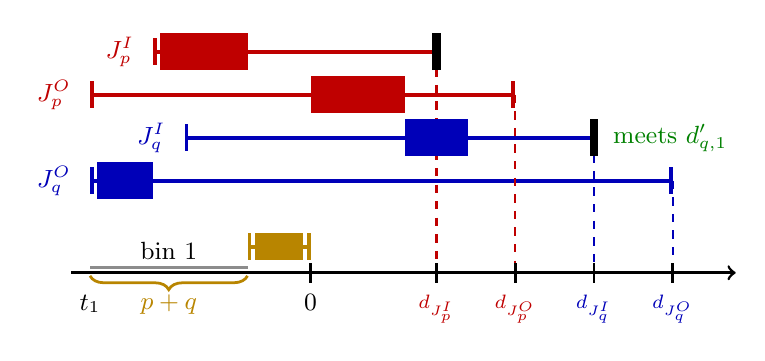
\begin{tikzpicture}[x=0.40cm,y=0.78cm]
  \def\ta{-7}
  \def\pw{3}\def\qw{2}
  % axis and bin 1, with its separator
  \draw[line width=1pt,->] (-7.6,0) -- (13.5,0);
  \draw[line width=1pt] (0,-0.16) -- (0,0.16);
  \node[font=\small,anchor=north] at (0,-0.2) {$0$};
  \node[font=\small,anchor=north] at (\ta,-0.2) {$t_1$};
  \draw[mygray,line width=1pt] (\ta,0.08) -- (\ta+5,0.08);
  \node[font=\small] at (\ta+2.5,0.35) {bin $1$};
  \fill[mysolutioncolor] (\ta+5.25,0.2) rectangle (\ta+6.75,0.65);
  \draw[mysolutioncolor,line width=1.4pt,|-|] (\ta+5,0.425) -- (\ta+7,0.425);
  \draw[decorate,decoration={brace,mirror,amplitude=5pt},color=mysolutioncolor,
        line width=1pt] (\ta,-0.05) -- (\ta+5,-0.05);
  \node[font=\small,text=mysolutioncolor,anchor=north] at (\ta+2.5,-0.2) {$p+q$};
  % the pair's quad: four availability windows
  \draw[myred,line width=1.4pt,|-|]  (-5,3.6) -- (4,3.6);
    \node[font=\small,anchor=east,text=myred]  at (-5.3,3.6) {$J^{I}_{p}$};
  \draw[myred,line width=1.4pt,|-|]  (\ta,2.9) -- (6.5,2.9);
    \node[font=\small,anchor=east,text=myred]  at (\ta-.3,2.9) {$J^{O}_{p}$};
  \draw[myblue,line width=1.4pt,|-|] (-4,2.2) -- (9,2.2);
    \node[font=\small,anchor=east,text=myblue] at (-4.3,2.2) {$J^{I}_{q}$};
  \draw[myblue,line width=1.4pt,|-|] (\ta,1.5) -- (11.5,1.5);
    \node[font=\small,anchor=east,text=myblue] at (\ta-.3,1.5) {$J^{O}_{q}$};
  \draw[myred,line width=0.8pt,dashed] (4,3.6) -- (4,0);
  \draw[line width=1pt] (4,-0.16) -- (4,0.16);
  \node[font=\scriptsize,anchor=north,text=myred] at (4,-0.2) {$d_{J^I_p}$};
  \draw[myred,line width=0.8pt,dashed] (6.5,2.9) -- (6.5,0);
  \draw[line width=1pt] (6.5,-0.16) -- (6.5,0.16);
  \node[font=\scriptsize,anchor=north,text=myred] at (6.5,-0.2) {$d_{J^O_p}$};
  \draw[myblue,line width=0.8pt,dashed] (9,2.2) -- (9,0);
  \draw[line width=1pt] (9,-0.16) -- (9,0.16);
  \node[font=\scriptsize,anchor=north,text=myblue] at (9,-0.2) {$d_{J^I_q}$};
  \draw[myblue,line width=0.8pt,dashed] (11.5,1.5) -- (11.5,0);
  \draw[line width=1pt] (11.5,-0.16) -- (11.5,0.16);
  \node[font=\scriptsize,anchor=north,text=myblue] at (11.5,-0.2) {$d_{J^O_q}$};
  \draw[line width=3pt] (4,3.3) -- (4,3.9);
  \draw[line width=3pt] (9,1.9) -- (9,2.5);
  % the schedule: inner short + inner long parked in the bin,
  % outer long + outer short running after time 0
  \fill[myblue] (\ta+.22,1.2)     rectangle (\ta+\qw,1.8);
  \fill[myred]  (\ta+\qw+.22,3.3) rectangle (\ta+\qw+\pw,3.9);
  \fill[myred]  (0,2.6)   rectangle (\pw,3.2);
  \fill[myblue] (\pw,1.9) rectangle (\pw+\qw,2.5);
  \node[font=\small,anchor=west,text=mygreen] at (9.3,2.2) {meets $d'_{q,1}$};
\end{tikzpicture}

\caption{Bin $1$, pinned by its separator (amber), holding the inner short
job $J^I_q$ and the inner long job $J^I_p$; the outer long job $J^O_p$ and
outer short job $J^O_q$ run after time $0$, and $J^I_q$ meets its early
deadline $d'_{q,1}$.}
\label{fig:stacked}
\end{figure}

\begin{proposition}[The Construction Is Correct]
% lax begin Lax391470Proofs.StackedNumbering.correct
For job lengths $p>q\ge 1$, an ordered instance of $\AUX(p,q)$ has a solution
exactly when the stacked instance has a feasible schedule.
% lax end
\end{proposition}

\begin{proposition}
% lax begin Lax391470Proofs.StackedNumbering.lengthsIn
The stacked instance uses only the job lengths $p$ and $q$.
% lax end
\end{proposition}

\begin{proposition}[The Numbers Stay Small]
% lax begin Lax391470Proofs.StackedNumbering.times_le
If every release time and deadline of an ordered instance $A$ is at most
$T$, then every release time and deadline of the stacked instance is within
$T+(p+2q)N$ of $0$, where $N$ is the number of pending pairs.
% lax end
\end{proposition}
\end{proof}

Together with Proposition~\ref{prop:sattimes}'s bound on $\AUX(p,q)$'s own numbers,
this bounds every number produced by composing the two reductions by a
polynomial in the size of the original formula, since $p$ and $q$ are fixed
constants, the ingredient Elffers and de Weerdt's source uses to call the
hardness \emph{strong}.

As for Lemma~\ref{lem:lemma2}, three separate proofs give, respectively,
% lax begin Lax391470Proofs.Reduce.lemma1_reduce_correct
the reduction's correctness,
% lax end
% lax begin Lax391470Proofs.L1Final.reduce_polyTime
its polynomial running time,
% lax end
and
% lax begin Lax391470Proofs.Hardness.aux_manyOne_twoLengths
the many-one reduction Lemma~\ref{lem:lemma1} states.
% lax end

\section{Integer Start Times}

\begin{proposition}
% lax begin Lax391470.IntegralStartTimes
A scheduling instance is schedulable by a real-valued start-time assignment
exactly when it is schedulable by an integer one.
% lax end
\end{proposition}
\begin{proof}
% lax begin Lax391470Proofs.IntegralStartTimes.realSchedulable_iff
Rounding every start time up to the next integer only shortens the gap to
each job's deadline, and keeps execution intervals disjoint because every
release time and deadline is already an integer.
% lax end
This settles a remark Elffers and de Weerdt make in passing: nothing is lost
by restricting Definition~\ref{def:scheduling} to integer schedules, as the rest of
this paper does.
\end{proof}

\section{Putting It Together}

Composing Lemma~\ref{lem:lemma2} and Lemma~\ref{lem:lemma1} gives Theorem~\ref{thm:main}'s
NP-hardness:
\begin{itemize}
\item % lax begin Lax391470Proofs.Hardness.twoLengths_npHard
every language in \NP{} many-one reduces to scheduling on $\{p,q\}$ through
$\AUX(p,q)$;
% lax end
\end{itemize}
and, with membership, the theorem itself:
\begin{itemize}
\item % lax begin Lax391470Proofs.Hardness.twoLengths_npComplete
scheduling on the lengths $\{p,q\}$ is \NP-complete.
% lax end
\end{itemize}

\section{Formalization Notes}

Hardness rests on the archive's own proof of the Cook--Levin theorem, not on
a literature axiom: every language in \NP{} many-one reduces to
satisfiability as a cited result of
% lax begin lax-429075
\textsc{the Cook--Levin Theorem},
% lax end
composed here with the two reductions above. The polynomial-time bounds of
Lemma~\ref{lem:lemma2} and Lemma~\ref{lem:lemma1} are proved by exhibiting explicit
programs on
% lax begin lax-808846
\textsc{the Word RAM}
% lax end
and transferring their running time to Turing-machine polynomial time via
% lax begin lax-759944
the proved equivalence of the two models;
% lax end
composing the resulting machines over possibly different alphabets uses a
polynomial-time Turing-machine composition proved in
% lax begin lax-434930
\textsc{Classical Complexity Classes}.
% lax end

\section{Discussion}

Single-machine scheduling with release times and deadlines is
polynomial-time solvable when every job has the same length, and remains so
when the lengths are drawn from $\{1,p\}$ for any $p$~\cite{Sgall12}.
Theorem~\ref{thm:main} shows that this tractability is fragile: once both lengths
exceed $1$, the problem is \NP-complete, for every fixed pair $p>q>1$. Since
$p$ and $q$ are constants rather than part of the input, this rules out a
polynomial-time algorithm at any fixed pair of lengths, settling Sgall's
open question and Mnich and van Bevern's Open Problem 3
(Observation~\ref{obs:paranphard}). The dividing line between tractable and
\NP-complete sits exactly at excluding the unit length.

\clearpage
\begin{thebibliography}{9}
\bibitem{EdW17}
J.~Elffers and M.~de Weerdt.
\newblock Scheduling with Two Non-Unit Job Lengths Is NP-Complete.
\newblock arXiv:1412.3095, 2017.
\newblock \url{https://doi.org/10.48550/arXiv.1412.3095}.
\bibitem{Cook71}
S.~A. Cook.
\newblock The Complexity of Theorem-Proving Procedures.
\newblock In \emph{Proceedings of the Third Annual ACM Symposium on Theory of
Computing}, 151--158, 1971.
\newblock \url{https://doi.org/10.1145/800157.805047}.
\bibitem{Sgall12}
J.~Sgall.
\newblock Open Problems in Throughput Scheduling.
\newblock In \emph{Algorithms, ESA 2012}, 2--11, 2012.
\newblock \url{https://doi.org/10.1007/978-3-642-33090-2_2}.
\bibitem{Vakhania04}
N.~Vakhania.
\newblock Single-Machine Scheduling with Release Times and Tails.
\newblock \emph{Annals of Operations Research} 129:253--271, 2004.
\newblock \url{https://doi.org/10.1023/B:ANOR.0000030692.69147.e2}.
\bibitem{Mnich18}
M.~Mnich and R.~van Bevern.
\newblock Parameterized Complexity of Machine Scheduling: 15 Open Problems.
\newblock \emph{Computers \& Operations Research} 100:254--261, 2018.
\newblock \url{https://doi.org/10.1016/j.cor.2018.07.020}.
\end{thebibliography}

\end{document}
